\documentclass[xcolor=svgnames]{beamer}
% ,handout

\usefonttheme{professionalfonts} % using non standard fonts for beamer

\usepackage[utf8]    {inputenc}
\usepackage[T1]      {fontenc}
\usepackage[english] {babel}
\usepackage{graphicx}
\usepackage{fancyvrb}

\usepackage{amsmath,amsfonts,graphicx}
\usepackage{beamerleanprogress}

\graphicspath{{./}}

\title
[Scala Collections \hspace{2em}]
{Scala Collections \\ How many ways are there to say \\ "Multiple Things"}

\author
[Julian Bieber]
{Julian Bieber}

\date
{\today}


\begin{document}

    \maketitle

    \section{Collections Trivia}
    \begin{frame}
    {Collections Trivia}
        \begin{figure}
            \centering
            
\includegraphics[\textwidth]{trivia.pdf}
        \end{figure}
    \end{frame}

    \begin{frame}[fragile] % example1
    {Sequence}
        \begin{Verbatim}[formatcom=\sffamily]
val sequence = Seq(1, 2, 3, 4, 5)
println(sequence)
        \end{Verbatim}

        \noindent\makebox[\linewidth]{\rule{\paperwidth}{0.4pt}}

        \pause

        \begin{Verbatim}[formatcom=\sffamily]
List(1, 2, 3, 4, 5)
        \end{Verbatim}
    \end{frame}

    \begin{frame}[fragile] % example2
    {Stream}
        \begin{Verbatim}[formatcom=\sffamily]
val stream = Stream(1, 2, 3, 4, 5)
println(stream)
val seq: Seq[Int] = stream.toSeq
seq.map(println)
        \end{Verbatim}

        \noindent\makebox[\linewidth]{\rule{\paperwidth}{0.4pt}}

        \pause

        \begin{Verbatim}[formatcom=\sffamily]
Stream(1, ?)
1
        \end{Verbatim}
    \end{frame}

    \begin{frame}[fragile] % example3
    {Stream Consumption}
        \begin{Verbatim}[formatcom=\sffamily]
val stream = Stream(1, 2, 3)
stream.foreach(println)
val streamPlusOne = stream.map(_ + 1)
println(stream.size)
streamPlusOne.foreach(println)
        \end{Verbatim}

        \noindent\makebox[\linewidth]{\rule{\paperwidth}{0.4pt}}

        \pause

        \begin{Verbatim}[formatcom=\sffamily]
1
2
3
3
2
3
4
        \end{Verbatim}
    \end{frame}

    \begin{frame}[fragile] % example4
    {Sequence Order of Execution}
        \begin{Verbatim}[formatcom=\sffamily]
Seq(1, 2, 3).map{ i =>
    println("method1", i)
    i
}.map{ i =>
    println("method2", i)
    i
}
        \end{Verbatim}

        \noindent\makebox[\linewidth]{\rule{\paperwidth}{0.4pt}}

        \pause

        \begin{Verbatim}[formatcom=\sffamily]
(method1,1)
(method1,2)
(method1,3)
(method2,1)
(method2,2)
(method2,3)
        \end{Verbatim}
    \end{frame}

    \begin{frame}[fragile] % example5
    {Stream Order of Execution}
        \begin{Verbatim}[formatcom=\sffamily]
Stream(1, 2, 3).map{ i =>
  println("method1", i)
  i
}.map{ i =>
  println("method2", i)
  i
}
        \end{Verbatim}

        \noindent\makebox[\linewidth]{\rule{\paperwidth}{0.4pt}}
(method1,1)
(method2,1)
        \pause

        \begin{Verbatim}[formatcom=\sffamily]

        \end{Verbatim}
    \end{frame}

    \begin{frame}[fragile] % example6
    {Stream.force?}
        \begin{Verbatim}[formatcom=\sffamily]
Stream(1, 2, 3).map{ i =>
  println("method1", i)
  i
}.map{ i =>
  println("method2", i)
  i
}.force
        \end{Verbatim}

        \noindent\makebox[\linewidth]{\rule{\paperwidth}{0.4pt}}

        \pause

        \begin{Verbatim}[formatcom=\sffamily]
(method1,1)
(method2,1)
(method1,2)
(method2,2)
(method1,3)
(method2,3)
        \end{Verbatim}
    \end{frame}

    \begin{frame}[fragile] % example7
    {Infinite Streams}
        \begin{Verbatim}[formatcom=\sffamily]
val stream = Stream.from(1).map{ i =>
  println("method1", i)
  i
}.map{ i =>
  println("method2", i)
  i
}

println(stream.sum)
        \end{Verbatim}

        \noindent\makebox[\linewidth]{\rule{\paperwidth}{0.4pt}}

        \pause

        \begin{Verbatim}[formatcom=\sffamily]
...
(method1,2517132)
(method2,2517132)

Exception: java.lang.OutOfMemoryError
        \end{Verbatim}
    \end{frame}

    \begin{frame}[fragile] % example8
    {Infinite Iterators}
        \begin{Verbatim}[formatcom=\sffamily]
val iterator = Stream.from(1).map{ i =>
  println("method1", i)
  i
}.map{ i =>
  println("method2", i)
  i
}.toIterator

println(iterator.sum)
        \end{Verbatim}

        \noindent\makebox[\linewidth]{\rule{\paperwidth}{0.4pt}}

        \pause

        \begin{Verbatim}[formatcom=\sffamily]
...
(method1,2517132)
(method2,2517132)
...
        \end{Verbatim}
    \end{frame}

    \section{Type Hierarchy}

    \begin{frame}
    {Type Hierarchy}
        \begin{figure}
            \centering
            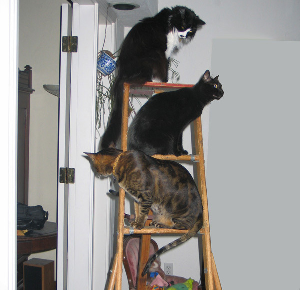
\includegraphics[\textwidth]{hierarchy.pdf}
        \end{figure}
    \end{frame}

    \begin{frame}[fragile]
    {Immutabe}
        \begin{figure}
            \centering
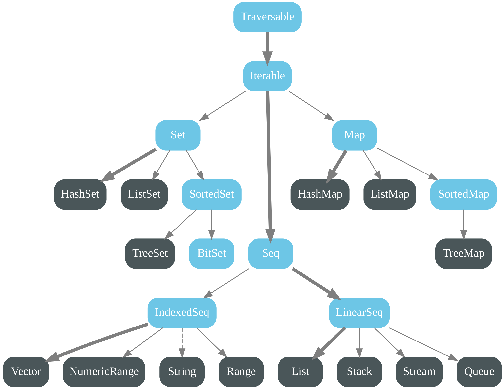
\includegraphics[width=0.9\textwidth]{collections-immutable-diagram.pdf}
        \end{figure}
    \end{frame}

    \begin{frame}
    {Array}
        \begin{itemize}
            \item slow prepend/append
            \item very fast random access ($O(1)$)
            \item contiguous locality
            \item strict
        \end{itemize}
    \end{frame}

    \begin{frame}
    {Vector}
        \begin{itemize}
            \item fast random access ($O(c)$)
            \item fast append/prepend ($O(c)$)
            \item good but not contiguous locality
            \item strict
        \end{itemize}
    \end{frame}

    \begin{frame}
    {List}
        \begin{itemize}
            \item very fast prepend ($O(1)$)
            \item very fast head access ($O(1)$)
            \item single linked $\Rightarrow$ slow random access ($O(n)$)
            \item bad locality
            \item strict
        \end{itemize}
    \end{frame}

    \begin{frame}
    {Stream}
        \begin{itemize}
            \item List with lazy tail
            \item while something holds the head it can not be GC'ed
            \item will not be consumed by iterating (while something hold the head)
            \item not strict
        \end{itemize}
    \end{frame}

    \section{Views}

    \begin{frame}[fragile]
    {Concept of a View}
        \begin{itemize}
            \item calling view on a collection makes it non strict
            \item modifications can be applied as usual (map, filter, \textellipsis)
            \item however they are not evaluated yet \pause
            \item force applies the changes
            \item better memory foodprint
        \end{itemize}
    \end{frame}

    \begin{frame}[fragile]
    {Scala SeqView}
        \begin{itemize}
            \item Signature: SeqView[+A, +Coll]
            \item Represents a view to Coll[+A]
            \item chaining maps without creating new collections
            \item $\Rightarrow$ less memory consumption \pause
            \item $\Rightarrow$ less GC activity \pause
            \item $\Rightarrow$ faster
        \end{itemize}
    \end{frame}

    \section{Benchmarks}

    \begin{frame}
    {Benchmarks}
        \begin{figure}
            \centering
            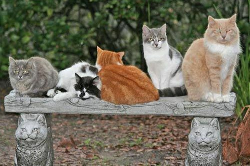
\includegraphics[\textwidth]{cats.pdf}
        \end{figure}
    \end{frame}



\end{document}

